%  LaTeX support: latex@mdpi.com
%  In case you need support, please attach any log files that you could have, and specify the details of your LaTeX setup (which operating system and LaTeX version / tools you are using).

%=================================================================

% LaTeX Class File and Rendering Mode (choose one)
% You will need to save the "mdpi.cls" and "mdpi.bst" files into the same folder as this template file.

%=================================================================

\documentclass[journal,article,accept,moreauthors,pdftex,12pt,a4paper]{mdpi}
\usepackage{tikz}
\usepackage{tikz-3dplot}
\usetikzlibrary{shapes,calc,positioning}
\tdplotsetmaincoords{60}{60}
\usepackage{amsmath}
\usepackage{graphicx,subcaption}
\usepackage{amssymb}
\usepackage{color}
\usepackage{float}

\newcommand{\red}[1]{\textbf{\color{red} ***ATT*** #1}}
\newcommand{\green}[1]{\textbf{\color{green} ***ATT*** #1}}


\usepackage{changes}
\definechangesauthor[name={Rafael}, color=blue]{raf}
\setremarkmarkup{(#2)}
\definechangesauthor[name={Luis}, color= magenta]{luis}
\setremarkmarkup{(#2)}

%--------------------
% Class Options:
%--------------------
% journal
%----------
% Choose between the following MDPI journals:
% actuators, administrativesciences, aerospace, agriculture, agronomy, algorithms, animals, antibiotics, antibodies, antioxidants, appliedsciences, arts, atmosphere, atoms, axioms, batteries, behavioralsciences, bioengineering, biology, biomedicines, biomolecules, biosensors, brainsciences, buildings, cancers, catalysts, cells, challenges, chemosensors, children, chromatography, climate, coatings, computation, computers, cosmetics, crystals, dentistryjournal, diagnostics, diseases, diversity, econometrics, economies, education, electronics, energies, entropy, environmentalsciences, environments, epigenomes, fibers, foods, forests, futureinternet, galaxies, games, gels, genealogy, genes, geosciences, healthcare, horticulturae, humanities, hydrology, informatics, information, inorganics, insects, ijerph, ijfs, ijms, ijgi, jcdd, jcm, jdb, jfb, jimaging, jof, joi, jlpea, jmse, jpm, jrfm, jsan, land, laws, life, lubricants, machines, marinedrugs, materials, mathematics, medicalsciences, membranes, metabolites, metals, microarrays, micromachines, microorganisms, minerals, molbank, molecules, nanomaterials, ncrna, nutrients, pathogens, pharmaceuticals, pharmaceutics, pharmacy, photonics, plants, polymers, processes, proteomes, publications, religions, remotesensing, resources, risks, robotics, safety, sensors, sinusitis, socialsciences, societies, sports, standards, sustainability, symmetry, systems, technologies, toxics, toxins, universe, vaccines, veterinarysciences, viruses, water
%---------
% article
%---------
% The default type of manuscript is article, but could be replaced by using one of the class options:
% article, review, communication, commentary, bookreview, correction, addendum, editorial, changes, supfile, casereport, comment, conceptpaper, conferencereport, meetingreport, discussion, essay, letter, newbookreceived, opinion, projectreport, reply, retraction, shortnote, technicalnote, creative
%----------
% submit
%----------
% The class option "submit" will be changed to "accept" by the Editorial Office when the paper is accepted. This will only make changes to the frontpage (e.g. the logo of the journal will get visible), the headings, and the copyright information. Journal info and pagination for accepted papers will also be assigned by the Editorial Office.
% Please insert a blank line is before and after all equation and eqnarray environments to ensure proper line numbering when option submit is chosen
%------------------
% moreauthors
%------------------
% If there is only one author the class option oneauthor should be used. Otherwise use the class option moreauthors.
%---------
% pdftex
%---------
% The option "pdftex" is for use with pdfLaTeX only. If eps figure are used, use the optioin "dvipdfm", with LaTeX and dvi2pdf only.

%=================================================================
\setcounter{page}{1}
\lastpage{x}
\doinum{10.3390/------}
\pubvolume{xx}
\pubyear{2015}
%\externaleditor{Academic Editor: xx}
\history{Received: xx / Accepted: xx / Published: xx}
%------------------------------------------------------------------
% The following line should be uncommented if the LaTeX file is uploaded to arXiv.org
%\pdfoutput=1

%=================================================================

% Add packages and commands to include here
% The amsmath, amsthm, amssymb, hyperref, caption, float and color packages are loaded by the MDPI class.
%\usepackage{graphicx}
%\usepackage{subfigure,psfig}

%=================================================================
%% Please use the following mathematics environments:
%\theoremstyle{mdpi}
%\newcounter{thm}
%\setcounter{thm}{0}
%\newcounter{ex}
%\setcounter{ex}{0}
%\newcounter{re}
%\setcounter{re}{0}
%\newtheorem{Theorem}[thm]{Theorem}
%\newtheorem{Lemma}[thm]{Lemma}
%\newtheorem{Characterization}[thm]{Characterization}
%\newtheorem{Proposition}[thm]{Proposition}
%\newtheorem{Property}[thm]{Property}
%\newtheorem{Problem}[thm]{Problem}
%\newtheorem{Example}[ex]{Example}
%\newtheorem{Remark}[re]{Remark}
%\newtheorem{Corollary}[thm]{Corollary}
%\newtheorem{Definition}[thm]{Definition}
%% For proofs, please use the proof environment (the amsthm package is loaded by the MDPI class).

%=================================================================

% Full title of the paper (Capitalized)
\Title{Comparing probabilistic predictive models applied to football}

% Authors (Add full first names)
\Author{Marcio A. Diniz $^{1,}$*, Rafael Izbicki $^{1}$, Danilo Lopes $^{1}$ and Luis Ernesto Salasar $^{1}$}

% Affiliations / Addresses (Add [1] after \address if there is only one affiliation.)
\address{%
$^{1}$ Department of Statistics, Federal University of S\~ao Carlos, Rod. Washington Luis, km 235, S. Carlos, Brazil}

% Contact information of the corresponding author (Add [2] after \corres if there are more than one corresponding author.)
\corres{marcio.alves.diniz@gmail.com, (+5516) 3351-9387.}

% Abstract (Do not use inserted blank lines, i.e. \\)
\abstract{We create three simple multinomial-Dirichlet models and compare them to two well-known sophisticated statistical models for association football (soccer) predictions according to their performance in predicting the full-time results for the second round of the 2014 Brazilian first division championship.  The predictive models are compared using three proper scoring rules, the proportion of errors and the calibration assessment. Our results show similar predictive performances for all the five methods, thus discouraging the use of overcomplicated models for match result forecast.}

% Keywords: add 3 to 10 keywords
\keyword{predictive inference; probabilistic prediction; Bayesian inference; scoring rules}

% The fields PACS, MSC, and JEL may be left empty or commented out if not applicable
%\PACS{}
%\MSC{}
%\JEL{}

% If this is an expanded version of a conference paper, please cite it here: enter the full citation of your conference paper, and add $^\dagger$ in the end of the title of this article.
%\conference{}

\begin{document}

%%%%%%%%%%%%%%%%%%%%%%%%%%%%%%%%%%%%%%%%%%

\section{Introduction}

The famous saying of John von Neumann: {\it ``With four parameters I can fit an elephant, and with five I can make him wiggle his trunk''} is a perhaps just a humorous version of Ockham's razor:
{\it``Entities are not to be multiplied without necessity''}, but illustrates very well a principle that is not often followed by researchers, especially when building predictive models.
This is true also in the literature of probabilistic sports predictions, particularly regarding models devoted to football or soccer\footnote{Henceforth, football.} predictions.

Bothered by such concerns, our goal was to answer the following question: is it possible, using a simple probabilistic model, to predict results of football matches better than more sophisticated or complex models?
To answer this, we compared two sophisticated models that consider multiple covariates with simple multinomial-Dirichlet models that consider only the number of matches won, tied or lost by each team as inputs.
The models were tested for the second round of the Brazilian football championships of first division and compared using standard metrics or scoring rules.
We also used other criteria such as the proportion of matches that were predicted ``correctly'' by each model and a measure of calibration, both explained in detail below.
According to the adopted criteria, the simple models showed a similar predictive performance to the complex ones.

The predictions of the two benchmark models were published on Internet websites before every matchday, and are treated by us as black-box models (BB1 and BB2). 
We know that\footnote{One of the authors is responsible for one of these models and the other was described in a dissertation. See \cite{arruda2000}.} both models are based on Holgate bivariate Poisson regression considering as explanatory variables the home field advantage, attack and defense strength for each team, and provide the probabilities of all possible outcomes (home team wins, draws or loses) for each match.
Because both models are based on elaborate parametric assumptions, they are suitable for the comparison we are proposing: simple versus complex models\footnote{To be precise we would have to define what is a ``simple'' model and what is a ``complex'' model. Based on the opening quotations, one may say that the number of parameters defines the complexity of a model, which is not exactly the definition we will use, since we consider other criteria, like the interpretation of explanatory variables and mathematical structure of the statistical model.}.


There are several ways to score or classify predictions of categorical events that assume one result out of a discrete set of mutually exclusive possible outcomes, like football matches.
See \cite{constantinou} for a brief survey of such measures applied to football.
We decided to score the previsions for each match in terms of their distances from the truth, i.e. the verified event, once it has occurred, and chose the most used distances in the literature: Brier \cite{brier1950}, logarithmic and spherical.

This paper is organized as follows.
Section \ref{sec::experimental} describes the proposed models, Section \ref{sec::scoring} presents the scoring rules and criteria used in this work to classify the models.
Section \ref{sec::results} reports the performance of the models predicting 190 matches comprising the second round of the Brazilian championship of first division.
In Section \ref{sec::remarks} we discuss the results and close with proposals for future research.


%%%%%%%%%%%%%%%%%%%%%%%%%%%%%%%%%%%%%%%%%%

\section{The models: theoretical background}
\label{sec::experimental}
%% Only for the journal Gels: Please place the Experimental Section after the Conclusions

In the literature, statistical models devoted to the prediction of
football matches can be divided in two classes: models that make
assumptions about the number of goals each team scores
\citep{Maher82, Dixon97, Karlis2003} and models that make
assumptions about the categorical final outcome (win, draw or defeat
of the home team) \citep{Forrest2000, Koning2000, Brillinger2008,
Brillinger2009}. For a discussion of these two approaches see
\cite{Goddard2005}. The benchmark models considered in this work are
part of the first approach, while the models proposed by us are part
of the second one.

In this section we present the probabilistic justification for the
three proposed models and the predictive distribution of an upcoming
match of team $A$ (home team) versus $B$ (away team). The main idea
is to combine the past performance of both teams in different ways
in order to predict the outcome of the match. The predictions of the
two benchmark models were published before each matchday at
\url{http://chancedegol.uol.com.br} and
\url{http://www.previsaoesportiva.com.br}.

%%%%%%%%%%%%%%%%%%%%%%%%%%%%%%%%%%%%%%%%%%

\subsection{Multinomial-Dirichlet}
\label{sec::Mn_Dir}

We adopt a Bayesian approach to calculate the prediction probabilities of an upcoming match of team $T$ ($A$ or $B$) based on its past performance, i.e, the number of matches it has won, tied and lost.

Let us consider the outcome of each match of team $T$ as a categorical random quantity $X$ that may assume only the values $1$, $2$, $3$, where $1$ means win ($W$), $2$ draw ($D$) and $3$ loss ($L$).
Denoting by $\theta_1, \theta_2$ and $\theta_3$ ($\theta_3 = 1-\theta_1 - \theta_2$), the probabilities of win, draw and loss, respectively, the probability mass function of $X$ is
\[
P(X=x | \boldsymbol{\theta}) = \theta_1^{\mathbb{I}_{\{1\}}(x)}
\theta_2^{\mathbb{I}_{\{2\}}(x)}(1 - \theta_1 -
\theta_2)^{{\mathbb{I}_{\{3\}}}(x)}, \qquad x \in \mathcal{X},
\]

\noindent
where $\mathcal{X}=\{1,2,3\}$ is the support of $X$,
$\mathbb{I}_{\{i\}}(x)$ is the indicator function that assumes the
value 1 if $x$ equals $i$ and 0 otherwise, and $\boldsymbol{\theta}
= (\theta_1, \theta_2)$ belogns to $\boldsymbol{\Theta} =
\{(\theta_1,\theta_2)\in [0,1]^2: \theta_1+\theta_2 \leq 1 \}$, the 2-simplex.

Assuming that $n$ matches of team $T$, given $\boldsymbol{\theta}$, are i.i.d. quantities with the above categorical distribution, and denoting by $M_1$, $M_2$ and $M_3$ the number of matches won, tied or lost by team $T$, the random vector $(M_1, M_2, M_2)$ has multinomial distribution with parameters $n$ and $\boldsymbol{\theta}$ given by
\[
P(M_1=n_1,M_2=n_2,M_3=n_3| n, \boldsymbol{\theta})=
\frac{n!}{n_1!n_2!(n-n_1-n_2)!}\theta_1^{n_1}\theta_2^{n_2}(1-\theta_1-\theta_2)^{n-n_1-n_2},
\]
\noindent 
where $n_1 + n_2 + n_3 = n$.

Our goal is to compute the predictive posterior distribution of the
upcoming match, $X_{n+1}$, that is,
$P(X_{n+1}=x|M_1=n_1,M_2=n_2,M_3=n_3)$, $x\in\mathcal{X}$. Using
Bayesian inference this probability can be easily computed as
follows. Suppose that $\boldsymbol{\theta}$ has Dirichlet prior distribution
with parameter $(\alpha_1,\alpha_2,\alpha_3)$, denoted
$\mathcal{D}(\alpha_1,\alpha_2,\alpha_3)$, with density function
\[
\pi(\boldsymbol{\theta}|\alpha)=\frac{\Gamma(\alpha_1+\alpha_2+\alpha_3)}{\Gamma(\alpha_1)\Gamma(\alpha_2)\Gamma(\alpha_3)}\theta_1^{\alpha_1-1}\theta_2^{\alpha_2-1}(1-\theta_1-\theta_2)^{\alpha_3-1}
\]
\noindent for $\alpha_1$, $\alpha_2$, $\alpha_3 > 0$, then the
posterior distribution of $\boldsymbol{\theta}$ is
$\mathcal{D}(n_1+\alpha_1,n_2+\alpha_2,n_3+\alpha_3)$. Thus, the
predictive distribution of $X_{n + 1}$ is given by the
integral
$$
P(X_{n + 1} = x | M_1 = n_1, M_2 = n_2, M_3 = n_3) = \int_{\boldsymbol{\Theta}} P(X_{n
+ 1} = x | \boldsymbol{\theta}) \pi(\boldsymbol{\theta} | M_1 = n_1, M_2 = n_2, M_3
= n_3) d\boldsymbol{\theta},
$$
which leads to the following probabilities of win, tie and loss:
\begin{align*}
P(X_{n+1} = 1 | M_1=n_1,M_2=n_2,M_3=n_3) &=
\frac{n_1+\alpha_1}{n+\alpha}\\
& \\
P(X_{n+1} = 2 | M_1=n_1,M_2=n_2,M_3=n_3) &=
\frac{n_2+\alpha_1}{n+\alpha} \\
& \\
P(X_{n+1} = 3 | M_1=n_1, M_2=n_2, M_3=n_3) &=
\frac{n_3+\alpha_1}{n+\alpha}
\end{align*}
\noindent where $\alpha=\alpha_1+\alpha_2+\alpha_3$.

In this work we used the uniform prior on the 2-simplex, i.e. $\mathcal{D}(1,1,1)$. 
This is not a restrictive prior because, since we predicted only the second round of the championship, the counts of the first round were used to update this prior---thanks to the conjugacy property of Dirichlet priors---and we may say that the actual prior we used is therefore the number of matches won, tied or lost by each team added by one.
If we had started our predictions in the first round, this prior would not have given 
a good predictive performance, but in this case we could have used team rankings such the ones provided by federations and leagues to assess a more realistic prior for each team instead.

Before we explain and illustrate the proposed models with an example, we make two further remarks.
The first one is that we will separately consider home and away games for each team. This will allow us to take into account the different performances under those conditions.
The second remark is that the prediction of an upcoming match between $A$ and $B$ can be done using
the past performance of either team $A$ or $B$.
To solve this problem, a compromise between the two predictive distributions was adopted. 
The next subsections \ref{sec::Mn_Dir1}, \ref{sec::Mn_Dir2} and \ref{sec::Mn_Dir3} present three different possible solutions.


\subsection{Model One: Multinomial-Dirichet $1$}
\label{sec::Mn_Dir1}

The model $Mn-Dir_1$ is defined as a mixture with equal weights of two Dirichlet distributions: the posterior distributions of teams $A$ and $B$. 
Since teams $A$ and $B$ are the home and away teams, respectively, the two posterior distributions to be mixed are: (i) one considering only the matches $A$ played at home; (ii) another considering only the matches $B$ played away. 
The relevant past performance of teams $A$ and $B$ will be summarized, respectively, by the count vectors ${\bf h} = (h_1, h_2, h_3)$ (team $A$ at home) and ${\bf a} = (a_1, a_2, a_3)$ (team $B$ away), representing the numbers of matches won, tied and lost, respectively.

For instance, consider the match Gr\^emio versus Atl\'etico-PR played for matchday 20, at Gr\^emio stadium. Table \ref{tab:counts} displays the performances of both teams, home and away, after 19
matches. The relevant vector of counts to be used are ${\bf h}=(h_1,h_2,h_3)=(6,2,1)$ and ${\bf a}=(a_1,a_2,a_3)=(2,3,4)$. 
Therefore, Gr\^emio has a $\mathcal{D}(7,3,2)$ posterior for matches played at home and Atl\'etico has a $\mathcal{D}(3,4,5)$ posterior for matches played as visitor (recall that both priors were
$\mathcal{D}(1,1,1)$).

\begin{table}[!h]
\begin{center}
\begin{tabular}{lccccccccc}

\hline
 & \multicolumn{3}{c}{Home} & \multicolumn{3}{c}{Away}& \multicolumn{3}{c}{Overall} \\
\hline
\hline
Team & W & D & L & W & D & L & W & D & L\\
\hline
Gr\^emio & 6 & 2 & 1 & 3 & 2 & 5 & 9 & 4 & 6\\
Atl\'etico-PR & 4 & 4 & 2 & 2 & 3 & 4 & 6 & 7 & 6\\
\hline
\end{tabular}
\caption{Gr\^emio and Atl\'etico-PR counts after 19 matchdays (first round)}\label{tab:counts}
\end{center}
\end{table}

Thus, considering $X_{n + 1}$ the random outcome of this match with
respect to the home team (Gr\^{e}mio), the predictive probabilities
of $X_{n + 1}$ is obtained by equally weighting the two predictive
distributions, resulting
\begin{align*}
P(X_{n+1}=1|{\bf h}, {\bf a}) &=
\frac{1}{2}\left(\frac{h_1+\alpha_1}{h+\alpha}\right)+\frac{1}{2}\left(\frac{a_3+\alpha_3}{a+\alpha}\right)=0.5
\\
P(X_{n+1}=2|{\bf h}, {\bf a}) &=
\frac{1}{2}\left(\frac{h_2+\alpha_2}{h+\alpha}\right)+\frac{1}{2}\left(\frac{a_2+\alpha_2}{a+\alpha}\right)\simeq0.2917, \\
P(X_{n+1}=3|{\bf h}, {\bf a}) &= \frac{1}{2}
\left(\frac{h_3+\alpha_3}{h+\alpha}\right)+\frac{1}{2}\left(\frac{a_1+\alpha_1}{a+\alpha}\right)\simeq0.2083.
\end{align*}
\noindent where $h=h_1+h_2+h_3$ and $a=a_1+a_2+a_3$.

\subsection{Model Two: Multinomial-Dirichlet $2$}
\label{sec::Mn_Dir2}

The model $Mn-Dir_2$ is very similar to model $Mn-Dir_1$, but the
weights used to mix the posterior distributions are not the same.
Model $Mn-Dir_2$ weights the predictive distributions according to
the team ranks just before the match is played. In the illustrative
example, we know that after 19 matchdays, Gr\^emio was the $6^{th}$
place and Atl\'etico-PR the $11^{th}$. Therefore, we shall consider
the weights
\[w_1 = \frac{1/6}{1/6+1/11}=0.647 ~ ~ ~ ~ ~\text{and} ~ ~ ~ w_2 = \frac{1/11}{1/6+1/11}=0.353\]
\noindent for the Gr\^emio and Atl\'etico predicitive distributions,
respectively. Thus, the winning probability for Gr\^emio is
calculated as
\[P(X_{n+1}= 1|{\bf h}, {\bf a})=0.647\left(\frac{h_1+\alpha_1}{h+\alpha}\right)+0.353\left(\frac{a_3+\alpha_3}{a+\alpha}\right)=0.525,\]
\noindent and the other probabilities are computed similarly.

\subsection{Model 3: Multinomial-Dirichlet 3}
\label{sec::Mn_Dir3}

Model $Mn-Dir_3$ is essentially different from the
last two, because it combines the two different count vectors ${\bf
h} = (h_1, h_2, h_3)$ and ${\bf a} = (a_1, a_2, a_3)$ instead of the
predictive distributions. The main idea is to add the information
contained in both vectors. From the point of view of team $A$, this can
be done by considering a win of team $B$ as a ``negative event'' and a
loss of team $B$ as a ``positive event'', while a draw is
considered an ``indifferent event''. Applying this reasoning,
we define the combined vector ${\bf c} = (c_1, c_2, c_3)$ by $c_1 =
h_1 + a_3$, $h_2 = h_2 + a_2$, and $h_3 = h_3 + a_1$. Then, assuming that the vector ${\bf c} = (c_1, c_2, c_3)$, given $\boldsymbol{\theta}$, has multinomial distribution with parameters $n$ and
$\boldsymbol{\theta}$, the predictive distribution for $X_{n + 1}$ can
be obtained by the methods explained in subsection
\ref{sec::Mn_Dir}.

It is important to highlight that this model implicitly uses the strong assumption that, given $\boldsymbol{\theta}$, the matches of the home team, when playing in its stadium, and the matches of the visitor team, when playing away, are independent and identically distributed (reversing the result outcomes for team $B$).

Considering the example above, the combined vector ${\bf c}$ is given by ${\bf c}=(c_1,c_2,c_3)=(10,5,3)$, which leads to a posterior $\mathcal{D}(11,6,4)$ when considering the prior $\mathcal{D}(1,1,1)$.
The probability that Gr\^emio wins is therefore	
\[P(X_{n+1}=1|{\bf c})=\frac{c_1+\alpha_1}{c+\alpha}\simeq0.524
\]

\noindent
where $c=c_1+c_2+c_3$. The probabilities of drawing and losing are computed similarly.

\section{Scoring rules and calibration}
\label{sec::scoring}

How can we fairly distinguish better-informed states of knowledge from more poorly informed states?
A way of doing this is to use proper scoring rules for evaluating states of uncertain knowledge, where
the score may be interpreted as a numerical measure of how inaccurate was the prevision.

%More precisely, a scoring rule is a function of two variables (or vectors, matrices etc) that assigns a real number (score) to each possible outcome $X$ and its respective prevision value, $P(X)$.
%It is maximum for each $x$ when $x=P(X)$, and is nonincreasing both as $x$ departs from $P(X)$ (for each $P(X)$) and as $P(X)$ departs from $x$ (for each $x$).
%Thus, the best score is achieved when knowledge of $X$ is asserted as the value of $X$ itself, whatever it might be. Most of the scoring rules also exhibit an arbitrary normalizing feature such as $S[x,P(X)]=0$ for each $x$.

%Although many functions satisfy the criteria for a scoring rule specified above, not every scoring rule can be regarded as providing a fair assessment of the assertion $P(X)$, that is, not all scoring rules encourage honesty and accuracy in assessing numerical values for their previsions.
%Those that do encourage a fair assessment are named \emph{proper scoring rules} \cite{lad}.

%Say a forecaster's uncertainty about $X$ is $P_0$. A proper scoring rule is a scoring rule $S$ such that the prevision value $P(X)$ that minimizes $E_{P_0}[S(X,P(X))]$ is $P_0$.
%In other words, if one receives a reward $S(x,P(x))$ when $x$ happens and if $S$ is a proper scoring rule, then the highest expected reward is obtained by reporting one's  true uncertainty about $X$.
%The use of a proper scoring rule thus encourages the forecaster to be honest to maximize the expected reward.
%Moreover, this method leads automatically to an overall comparison between the outcomes of different personal evaluations concerned with the same totality of events.
%Therefore, the accumulated score may be considered a concrete measure of success of each forecaster or model.


More precisely, a scoring rule is a function of two variables (or vectors, matrices etc) that assigns a real number (score) to each possible outcome of $X$ and its respective prevision value, $P_X$, i.e. $P_X$ is the probability assigned to each possible outcome of $X$.
It is minimum for each $x$ when $P_X$ is such that $P_X(X=x)=1$, and is nondecreasing both as $x$ departs from $P_X$ (for each $P_X$) and as $P_X$ departs from $x$ (for each $x$).
Thus, the best score (the smaller value of the score) is achieved when knowledge of $X$ is asserted as the value of $X$ itself, whatever it might be\footnote{A scoring rule can also be defined to be such that a \emph{large} value of the score indicates good predictions.}.
%Most of the scoring rules also exhibit an arbitrary normalizing feature such as $S(x,P_X)=0$ for each $x$.

Although many functions satisfy the criteria for a scoring rule specified above, not every scoring rule can be regarded as providing a fair assessment of the assertion $P_X$, that is, not all scoring rules encourage honesty and accuracy in assessing numerical values for their previsions.
Those that do encourage a fair assessment are named \emph{proper scoring rules} \cite{lad}.

Say a forecaster's uncertainty about $X$ is $P_0$. A proper scoring rule is a scoring rule $S$ such that the prevision value $P_X$ that minimizes $E_{P_0}[S(X,P_X)]$ is $P_0$.
In other words, if one receives a penalty $S(x,P_X)$ when $x$ happens and if $S$ is a proper scoring rule, then the lowest expected penalty is obtained by reporting one's  true uncertainty about $X$.
The use of a proper scoring rule thus encourages the forecaster to be honest to minimize the expected penalty.
Moreover, this method leads automatically to an overall comparison between the outcomes of different personal evaluations concerned with the same totality of events and, therefore, the accumulated score may be considered a concrete measure of success of each forecaster or model.

In what follows, we describe in detail three proper scoring rules we use to asses the various models considered.
We also recall the concept of calibration and propose a way to measure the calibration degree of each model.

%Proper scoring rules are devised so that no one previses (expects) that intrigue in falsely announcing some other number as $P(X)$ would be advantageous for achieving a better score.
%The particular scoring functions we study in the generic form $S(X,P(X))$ can also be considered as utility functions, $U(X,P(X))$.
%The principle of asserting numerical values for $P(X)$ in such a way as to maximize your prevision for your score is equivalent to acting in a decision problem so as to maximize your expected utility.



\subsection{Brier scoring rule}

Let $P_X$ be a probability assignment for $X$.
The Brier score is given by
$$S(X;P_X)= \sum_{i}\mathbb{I}(X=x_i)(1- P_X(x_i))^2+\sum_{i}\mathbb{I}(X\neq x_i)P_X^2(x_i),$$
where $\mathbb{I}$ is the indicator function.


\begin{figure}
\begin{center}
\begin{tikzpicture}[scale=2,tdplot_main_coords,axis/.style={->},thick]

% -- remove these 3 lines if no axis is preferred
\draw[axis] (0, 0, 0) -- (1.4, 0, 0) node [right] {$p_1$};
\draw[axis] (0, 0, 0) -- (0, 1.4, 0) node [above] {$p_2$};
\draw[axis] (0, 0, 0) -- (0, 0, 1.4) node [above] {$p_3$};

\coordinate  (d1) at (1,0,0){};
\coordinate  (d2) at (0,1,0){};
\coordinate  (d3) at (0,0,1){};

% fill gray color with opacity
\fill[green!80,opacity=0.2] (d1) -- (d2) -- (d3)-- cycle;

\draw[-, green, thick] (0,0,1) -- (1,0,0);
\draw[-, green, thick] (0,0,1) -- (0,1,0);
\draw[-, green ,thick] (1,0,0) -- (0,1,0);

\node[fill,circle,inner sep=1.5pt,label={left:$(1,0,0)$}] at (d1) {};
\node[fill,circle,inner sep=1.5pt,label={south east:$(0,1,0)$}] at (d2) {};
\node[fill,circle,inner sep=1.5pt,label={left:$(0,0,1)$}] at (d3) {};

\draw[-latex,thick](d3) to [out=60,in=180] (1,1,2);

\node[label={right:away team wins}] at (1,1,2) {};

\draw[-latex,thick](d1) to [out=-90,in=180] (1,1,-1);

\node[label={right:home team wins}] at (1,1,-1) {};

\draw[-latex,thick](d2) to [out=-120,in=180] (1,1,-.25);

\node[label={right:draw}] at (1,1,-.25) {};

\node[fill, blue, circle,inner sep=1.5pt] at (0.25,0.35,0.40) {};

\draw[-latex,thick](0.25,0.35,0.40) to [out=90,in=180] (1,1,1.2);

\node[label={right:$(0.25,0.35,0.40)$: prediction}] at (1,.9,1.2) {};

\end{tikzpicture}
\caption{Bi-dimensional simplex (green surface): area of possible predictions}\label{fig:simplex}
\end{center}
\end{figure}


We interpret the Brier score in the case where one of three mutually exclusive outcomes happen, the case of a football match.
The green surface in Figure \ref{fig:simplex} represents the 2-simplex, i.e. the set of points such that $p_1+p_2+p_3=1$ for non-negative values of $p_1$, $p_2$ and $p_3$.
The triangle representing the simplex has sides of length $\sqrt{2}$ and its height is $\sqrt{6}/2$.
Drawing a similar equilateral triangle with height 1 and sides $2\sqrt{3}/3$, it is possible to represent all points of the simplex.
This new triangle is used to graphically display the predictions as internal points because the sum of the distances of every point inside it to each side, representing the probability of each event, is always one.

\begin{figure}[!ht]
    \centering
    \begin{subfigure}[b]{0.48\linewidth}        %% or \columnwidth
        \centering

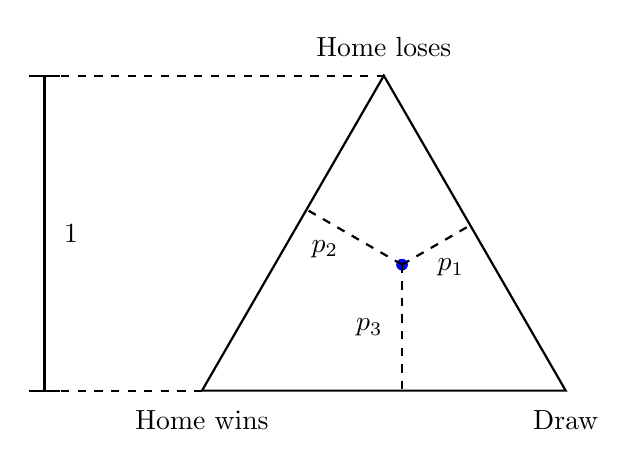
\begin{tikzpicture}[scale=4]
\draw [thick](0,0) -- (1.1547,0) -- (0.57735,1)-- (0,0);

\node[fill, blue, circle,inner sep=1.5pt] at (0.63509,0.40) {};

\draw[dashed,thick] (0.63509,0.40) -- (0.63509,0);
\draw[dashed,thick] (0.63509,0.40) -- (0.85159,0.525);
\draw[dashed,thick] (0.63509,0.40) -- (0.331976,0.575);

\node[label={left:$p_3$}] at (.63509,.2) {};
\node[label={below:$p_1$}] at (.79,.48) {};
\node[label={below:$p_2$}] at (.39,.54) {};

\node[label={below:Home wins}] at (0,0) {};
\node[label={below:Draw}] at (1.1547,0) {};
\node[label={above:Home loses}] at (0.57735,1) {};


\draw[-,thick] (-.5,0) -- (-.5,1);
\draw[-,thick] (-.45,0) -- (-.55,0);
\draw[-,thick] (-.45,1) -- (-.55,1);
\draw[dashed,thick] (-.5,1) -- (0.57735,1);
\draw[dashed,thick] (-.5,0) -- (0,0);


\node[label={right:$1$}] at (-.5,.5) {};


\end{tikzpicture}


        \caption{Normalized simplex: $p_1+p_2+p_3=1$}
        \label{fig:A}
    \end{subfigure}
    \begin{subfigure}[b]{0.48\linewidth}        %% or \columnwidth
        \centering

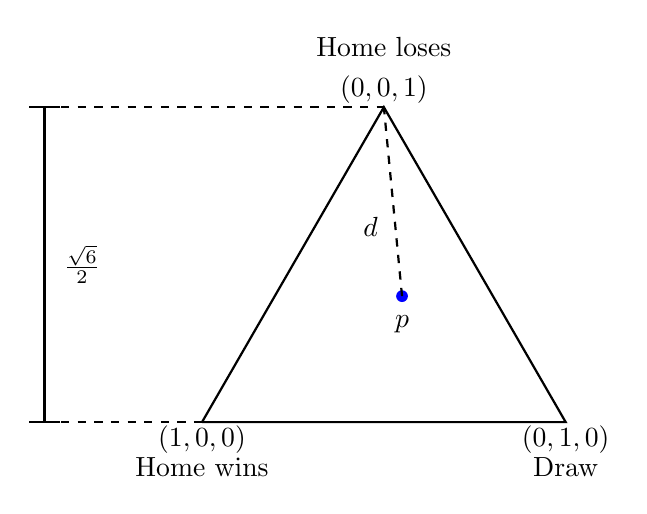
\begin{tikzpicture}[scale=4]
\draw [thick](0,0) -- (1.1547,0) -- (0.57735,1)-- (0,0);

\node[fill, blue, circle,inner sep=1.5pt] at (0.63509,0.40) {};
\node[label={below:$p$}] at (0.63509,0.40) {};

\node[label={left:$d$}] at (0.62,0.62) {};


\draw[dashed,thick] (0.63509,0.40) -- (0.57735,1);

\node[label={below:Home wins}] at (0,-0.05) {};
\node[label={below:Draw}] at (1.1547,-0.05) {};
\node[label={above:Home loses}] at (0.57735,1.1) {};

\node[label={below:$(1,0,0)$}] at (0,0.05) {};
\node[label={below:$(0,1,0)$}] at (1.1547,0.05) {};
\node[label={above:$(0,0,1)$}] at (0.57735,0.95) {};


\draw[-,thick] (-.5,0) -- (-.5,1);
\draw[-,thick] (-.45,0) -- (-.55,0);
\draw[-,thick] (-.45,1) -- (-.55,1);
\draw[dashed,thick] (-.5,1) -- (0.57735,1);
\draw[dashed,thick] (-.5,0) -- (0,0);

\node[label={right:$\frac{\sqrt{6}}{2}$}] at (-.5,.5) {};

\end{tikzpicture}


        \caption{Original simplex: used to compute the Brier score}
        \label{fig:B}
    \end{subfigure}
    \caption{Normalized and standard simplexes}
    \label{fig:norm_stand}
\end{figure}

The Brier score for the prediction $P_X=(0.25,0.35,0.40)$, assuming the home team loses, is therefore given by $d^2=(0-0.25)^2+(0-0.35)^2+(1-0.40)^2=0.545$. 
If the prediction was $P_X=(0,0,1)$, the score would be zero, the minimum for this rule.

It is useful to consider the score of what we will call {\it trivial prediction}: $(1/3,1/3,1/3)$.
This assessment will produce a Brier score of $2/3$, no matter what is the final result of the match, providing, thus, a threshold that a good model should consistently beat, meaning, for the Brier score, that the scores of its predictions should be smaller than $0.667$.  

%%%%%%%%%%%%%%%%%%%%%%%%%%%%%%%%%%%%%%%%%%


\subsection{Logarithmic scoring rule}

The logarithmic  score is given by
$$S(X;P_X)=- \sum_{i}\mathbb{I}(X=x_i)\ln(P_X(x_i)),$$

\noindent
which is the negative log likelihood of the event that occurred.

The logarithmic score for the prediction $P_X=(0.25,0.35,0.40)$, when the home team loses is therefore 
$-\ln(0.4)\approx 0.91$. 
If the prediction was $P_X=(0,0,1)$, the score would be zero, once again the minimum of this rule.
For the logarithmic score, the trivial prediction gives a score of approximately $1.098$.

\subsection{Spherical scoring rule}

The spherical score is given by
$$S(X;P_X)=- \frac{1}{\sqrt{\sum_i P_X^2(x_i)}}\sum_{i}\mathbb{I}(X=x_i)P_X(x_i),$$

\noindent
which is the negative likelihood of the event that occurred, normalized by the square-root of the sum of the assigned squared probabilities.

The spherical score for the prediction $P_X=(0.25,0.35,0.40)$, assuming the home team loses, is given by
$-0.4/\sqrt{0.25^2+0.35^2+0.40^2} \approx -0.68$.
If the prediction was $P_X=(0,0,1)$, the score would be $-1$ instead and, for this rule, the trivial prediction results in a score of approximately $-0.577$.

\subsection{Calibration and proportion of errors}
\label{sec::calib}

Besides scoring rules, there are other criteria used to assess the quality of different predictions. Here we explore two of them.

The first one is the proportion of errors made by the model or assessor. This is simply the proportion of mistakes made when considering the highest probability assessment.
More precisely, the proportion of errors of a given prediction $P_X$ is defined by
$$\frac{1}{n}\sum_{j=1}^n \mathbb{I}\left(X_j \neq \arg \max_{x} P_X(x_{j})\right),$$
where $X_j$ is the outcome of the $j$-th match and $P_X(x_{j})$ is the probability attributed to result $x\in\mathcal{X}=\{1,2,3\}$ for the $j$-th match.

The second concept we use is that of calibration \cite{Dawid}. Probability assertions are said to be well calibrated at the level of probability $p$ if the observed proportion of all propositions that are assessed with probability $p$ equals $p$.

Because we typically do not have several predictions with the same assigned probability $p$, we obtain a plot by smoothing (i.e., regressing) the indicator function of whether a given result happened as a function of the probability assigned for that result, that is, we estimate the probability that a event occurs given its assigned probability.
%, that is, we regress  
%$$\{ \mathbb{I}_{\{i\}}(X_j) \}_{j=1,\ldots,n;i=1,2,3} \mbox{ over } \{P_X(x_j)\}_{j=1,\ldots,n;i=1,2,3}$$
% for each event $A_i$, i.e., each possible outcome of each match
%that occurred.
The smoothing is done via smoothing splines \cite{wahba}, with tuning parameters chosen by cross-validation.


%A person's probability assertions are said to be well calibrated at the value $p$ if the limiting frequency of occurrence of events that are assessed with probability $p$, equals $p$.


\section{Results}
\label{sec::results}

We display only the results for the first division of the Brazilian football championship; 
we also analyzed the results for the second division, which yield similar conclusions.
Both divisions have 20 teams that play against each other twice (home and away) and the team with more points after all matches are played is declared champion.
The last four are relegated to a minor division and, in first division, the first four play Copa Libertadores (South America champions league) and in second division the first four are promoted to first division.
Therefore, in each championship there is a total of 380 matches, 190 in each round.

%\begin{table}[h]
%\begin{center}
%\begin{tabular}{ccccc}

%\hline
%Matchday & BB1 & $Mn-Dir_1$ & $Mn-Dir_2$ & $Mn-Dir_3$\\
%\hline
%\hline
%1$^{st}$ & 7.267 & 8.003 & 8.131 & 8.263 \\
%2$^{nd}$ & 5.633 & 6.073 & 6.119 & 6.057 \\
%3$^{rd}$ & 7.183 & 7.086 & 7.384 & 7.183 \\
%4$^{th}$ & 7.458 & 6.776 & 6.731 & 6.829 \\
%5$^{th}$ & 5.246 & 5.492 & 5.494 & 5.414 \\
%6$^{th}$ & 5.126 & 5.169 & 5.589 & 5.043 \\
%7$^{th}$ & 5.837 & 5.033 & 4.939 & 4.897 \\
%8$^{th}$ & 7.462 & 6.616 & 6.509 & 6.667 \\
%9$^{th}$ & 8.223 & 7.520 & 7.733 & 7.671 \\
%10$^{th}$ & 4.818 & 5.623 & 5.825 & 5.578 \\
%\hline
%Total & 118.00 & 117.68 & 119.33 & 117.70 \\
%\hline
%Mean & 0.6178 & 0.6161 & 0.6248 & 0.6162 \\

%\hline
%\end{tabular}
%\caption{Score of the ten first rounds and mean score per match after 191 matches}
%\end{center}
%\end{table}



%\begin{table}[h]
%\begin{center}
%\begin{tabular}{ccccc}
%
%\hline
%BB1 & $Mn-Dir_1$ & $Mn-Dir_2$ & $Mn-Dir_3$\\
%\hline
%\hline
%0.6011 & 0.6119 & 0.6159 & 0.6115\\
%\hline
%\multicolumn{4}{c}{Chance de gol historic mean (1998-2015): 0.5977}\\
%\hline
%\end{tabular}
%\caption{First and Second Divisions means}
%\end{center}
%\end{table}


Figure~\ref{fig::scores} displays the boxplots of the scores and proportion of errors of the predictive models considered.
%It also shows an horizontal line with the score of the trivial prediction.
According to all scoring rules, all methods have similar performance, and they are more accurate than the trivial prediction, displayed in the plots
as an horizontal line\footnote{None of the 95\% confidence intervals for the mean score contain the score given by the trivial prediction.}. The mean scores and their standard errors are displayed
in Table \ref{tab::brier}.


\begin{figure}[H]
  \centering
\includegraphics[page=1,scale=0.3]{futebolComparacaoModelosForPaper.pdf}
\includegraphics[page=2,scale=0.3]{futebolComparacaoModelosForPaper.pdf}\\
\includegraphics[page=3,scale=0.3]{futebolComparacaoModelosForPaper.pdf}
\includegraphics[page=4,scale=0.3]{futebolComparacaoModelosForPaper.pdf}
  \caption{Scores and proportion of errors of the various predictive methods. Horizontal line represents the score of the trivial prediction $(1/3,1/3,1/3)$.}
  \label{fig::scores}
\end{figure}


\begin{table}[H]
\begin{center}
\begin{tabular}{ccccccc}
\hline
Score & BB1 & BB2 & $Mn-Dir_1$ & $Mn-Dir_2$ & $Mn-Dir_3$ & Trivial \\
\hline
\hline
Brier &0.58 (0.02) & 0.59 (0.02)& 0.61 (0.02)& 0.61 (0.02) & 0.61  (0.02) & 0.67 \\
Logarithmic & 0.98 (0.03) & 0.99 (0.03) & 1.02 (0.03)  & 1.02 (0.03)  & 1.02 (0.03) & 1.10  \\
Spherical &  -0.64 (0.02)& -0.64 (0.02)& -0.62 (0.02)& -0.63 (0.02)& -0.63 (0.02)& -0.58\\
\hline
\end{tabular}
\caption{Mean scores and their standard errors for 190 matches of first division.}
\label{tab::brier}
\end{center}
\end{table}


Figure \ref{fig::entropy} presents the boxplots of the entropy of each prediction for the predictive models considered.\footnote{Recall
that the entropy of a prediction $(p_1,p_2,p_3)$ is given by $- \sum_{i=1}^3 p_i \log{p_i}$}
Since the entropy values are smaller than 1.09, the plots show that the predictions
are typically more informative than the trivial prediction. Nevertheless, all methods yielded similar entropies in average, that is,
none of them seem to provide more informative probabilities.



\begin{figure}[H]
  \centering
\includegraphics[page=10,scale=0.3]{futebolComparacaoModelosForPaper.pdf}
  \caption{Entropy of the predictions of the various methods. Horizontal line represents the entropy of the trivial prediction $(1/3,1/3,1/3)$.}
  \label{fig::entropy}
\end{figure}


We also evaluated how reasonable were the predictions by assessing the calibration of the methods considered, i.e., by evaluating how often events which have assigned probability $p$ (for each $0<p<1$) happened (Section \ref{sec::calib}).
If these probabilities are close to $p$, one concludes that the methods are well-calibrated.
Results are displayed in Figure \ref{fig::calibration}.
Because the curves we obtained are close to the identity ($45^{\text{o}}$ line), we conclude that all methods are well-calibrated, except perhaps BB1, in which events with both low and high estimated probabilities happen more often
than predicted.

In order to have a deeper understanding about the probabilities
given by each method, Figure \ref{fig::probMandante} displays the
estimated conditional probability that the home team wins assuming
the match will not be a tie.
All models assign higher probabilities to the home team, showing that they capture the well known fact known as home advantage, peculiar in football matches and in other sport competitions \cite{Pollard86, Clarke95, Nevill99}.
Morever, the outputs from the methods introduced in this paper are
less dispersed than those from the other models used in the
literature.


\begin{figure}[H] \centering
\includegraphics[page=5,scale=0.3]{futebolComparacaoModelosForPaper.pdf}
\includegraphics[page=6,scale=0.3]{futebolComparacaoModelosForPaper.pdf}\\
\includegraphics[page=7,scale=0.3]{futebolComparacaoModelosForPaper.pdf}
\includegraphics[page=8,scale=0.3]{futebolComparacaoModelosForPaper.pdf}
\includegraphics[page=9,scale=0.3]{futebolComparacaoModelosForPaper.pdf}
\caption{Calibration of the various predictive methods: estimates of
occurrence frequency obtained by smoothing splines, with 95\%
confidence bands. Black line is the identity $y=x$.}
\label{fig::calibration}
\end{figure}


\begin{figure}[H] \centering
\includegraphics[page=11,scale=0.4]{futebolComparacaoModelosForPaper.pdf}
\caption{Conditional probability that the home team wins given there
is no draw. Horizontal line indicates a 50\% probability.}
\label{fig::probMandante}
\end{figure}


We therefore conclude that all methods have similar predictive power, and none of them is more informative in average.
Nevertheless, all methods yielded better predictions than the trivial prediction, and they are well-calibrated.

\section{Final remarks}
\label{sec::remarks}

%De Finetti was a radical subjectivist and pragmatist about probability and did not believe that it even made sense to talk about credences as being ``accurate'' or ``inaccurate''.
%Like Ramsey and Savage, he offered pragmatic arguments for probabilism.
%As a result, de Finetti did not speak of ``measures of inaccuracy'' or ``measures of distance from the truth'': he used the terms ``scoring rule'' and ``loss function''.


%De Finetti used what is called the Brier score, which is just the (squared) Euclidean distance — i.e., the sum of the squared differences between credences and (the 0/1 numerical correlates of) truth values.

%In the statistical literature, football prediction models can be divided in two main approaches: (i) modeling the number of goals \citep{Maher82, Dixon97, Karlis2003} and (ii) modeling the final outcome (win, draw or lose) of the matches \citep{Forrest2000, Koning2000, Brillinger2008, Brillinger2009}. For a discussion of these two approaches see \cite{Goddard2005}.
Although our benchmark models were here defined as complex, we can find much more elaborate models in the literature, hindering the estimation and prediction processes.
Among them, we can cite those based on modeling the match as a stochastic process evolving through time \citep{Dixon98, Volf2009, Titman2015}, those allowing for the team performance parameters to
change along the season \citep{Rue2000, Crowder2002, Owen2011, Koopman2015} and those modeling dependence between number of goals by means of bivariate count distributions \citep{Dixon97, Karlis2003, McHale2007, McHale2011}.

%Although the benchmark models were here considered complex models, we can find in the literature much more elaborate models, hindering the estimation and prediction process. 
%Among those, we can cite those based on modeling the match as a stochastic process evolving through time \citep{Dixon98, Volf2009, Titman2015}, those allowing for the team performance parameters to change along the season \citep{Rue2000, Crowder2002, Owen2011, Koopman2015} and those modeling dependence between number of goals by means of bivariate count distributions \citep{Dixon97, Karlis2003, McHale2007, McHale2011}.

According to standard scoring rules and other criteria here adopted to qualify the predictions, our findings show that the predictive power of the three simple models was quite similar to the benchmark models.
%We compared the probabilistic predictions of three simple models with the ones provided by two more complex models for the second round of the 2014 Brazilian football championships of first and second divisions. 
This work thus indicates that while there has been a boom in the literature with the proposal of several fancy and involved models, especially in the era of big data, simple models can many times do
as well as their complex counterparts. 

This is often unnoticed by users of such methods, which leads to the overuse of models that are
hard to interpret and to implement, and that also require one to keep track of several covariates. We would call this phenomenon the {\it king's nudity}\footnote{In allusion to Anderson's {\it The
Emperor's New Clothes}, \cite{emperor}: ``But he isn't wearing anything at all!''.}, that is not, of course, always observed. 
In this spirit, since we have explored only the prediction of football matches, we would like to study if the same extends to other fields such as, for instance, weather or economics forecasts.

If, on the one hand, our findings appear as another supportive example of Ockham's razor, on the other they pose several questions about probabilistic prediction of sport events. 
In particular, based on the fact that the models have similar performance, one may ask: is there an irreducible ``randomness'' or ``degree of unpredictability'' implicit in these events?
Is this degree an indicator of how tight or leveled is the championship being studied?

A suggestion of future research is to answer these questions by considering more championships and models, and by comparing them using other scoring rules. 
Another direction we would like to address is to test other weighting methods in models 1 and 2 here
proposed, and to evaluate their impact on the predictive power of the resulting predictions.

Once more we would like to stress that, when trying to answer all these questions, one must remember perhaps the most practical statement of Ockham's razor: ``when you have two competing theories that make exactly the same predictions, the simpler one is the better.''
However, what to infer from known recorded measurements about the values of yet unrecorded measurements is the responsibility of each knowing person.
There is general agreement in evaluating the evidence that measured observations provide for yet unmeasured experiences, but there have been controversies among very respected scientists regarding what conclusions are to be drawn from observations.

%%%%%%%%%%%%%%%%%%%%%%%%%%%%%%%%%%%%%%%%%

%\acknowledgments{Acknowledgments}

%Main text.

%%%%%%%%%%%%%%%%%%%%%%%%%%%%%%%%%%%%%%%%%

%\authorcontributions{Author Contributions}

%Main text.

%%%%%%%%%%%%%%%%%%%%%%%%%%%%%%%%%%%%%%%%%

%\conflictofinterests{Conflicts of Interest}

%State any potential conflicts of interest here or ``The authors declare no conflict of interest''.

%=================================================================
% References: Variant A
%=================================================================
% Back Matter (References and Notes)
%----------------------------------------------------------
% Style and layout of the references
\bibliographystyle{mdpi}
\makeatletter
\renewcommand\@biblabel[1]{#1. }
\makeatother

\begin{thebibliography}{999} % if there are less than 10 entries, enter a one digit number

% Reference 1
%\bibitem{ref-journal}
%Lastname, F.; Author, T. The title of the cited article. {\em Journal Abbreviation} {\bf 2008}, {\em 10}, 142-149.

% Reference 2
%\bibitem{ref-book}
%Lastname, F.F.; Author, T. The title of the cited contribution. In {\em The Book Title}; Editor, F., Meditor, A., Eds.; Publishing House: City, Country, 2007; pp. 32-58.


\bibitem{arruda2000}
Arruda, M. L. {\em Poisson, Bayes, Futebol e De Finetti}, M. A. dissertation (in Portuguese), University of S\~ao Paulo, 2000.

\bibitem{brier1950}
Brier, G. Verification of forecasts expressed in terms of probability. {\em Monthly Weather Review} {\bf 1950}, {\em 78}, 1-3.

\bibitem{Brillinger2008}
Brillinger, D. R. Modelling game outcomes of the Brazilian 2006
series A championship as ordinal-valued. {\em Brazilian Journal of Probability and Statistics} {\bf 2008}, {\em 22}, 89-104.

\bibitem{Brillinger2009}
Brillinger, D. R. An analysis of Chinese Super League partial
results. {\em Science in China Series A} {\bf 2009}, {\em 52},
1139-1151.

\bibitem{constantinou}
Constantinou, A. and Fenton, N. E. Solving the problem of inadequate scoring rules for assessing probabilistic football forecast models. {\em Journal of Quantitative Analysis in Sports} {\bf 2012}, {\em 8}, manuscript 1418.

\bibitem{Clarke95}
Clarke, S. R.; Norman, J. N. Home ground advantage of individual clubs in English soccer. {\em Journal of the Royal Statistical Society - Series D} {\bf 1995} ,
{\em 44}, 509-521.

\bibitem{Crowder2002} Crowder, M.; Dixon, M.; Ledford, A.; Robinson, M. Dynamic modelling and prediction of English Football League matches for betting. {\em Journal of the Royal
Statistical Society - Series D} {\bf 2002}, {\em 51}, 157-168.

\bibitem{Dawid} Dawid, A. P. The well-calibrated Bayesian. 
{\em Journal of the American Statistical Association} {\em 1982}, {\em 77}, 605-610.

\bibitem{Dixon97} Dixon, M. J.; Coles, S. C. Modelling association football scores and inefficiencies in the football betting market. {\em Applied Statistics} {\bf 1997}, {\em 46}, 265-280.

\bibitem{Dixon98} Dixon, M. J.; Robinson, M. E. A Birth Process Model for Association Football Matches. {\em Journal of the Royal Statistical Society - Series D}
{\bf 1998}, {\em 47}, 523-538.

\bibitem{emperor}
Andersen, H.  C. The emperor's new clothes. Genesis Publishing Pvt Ltd, 1987.

\bibitem{Forrest2000} Forrest, D.; Simmons, R. Making up the results: The work
of the football pools panel, 1963-1997. {\em Journal of the Royal Statistical Society - Series D} {\bf 2000}, {\em 49}, 253-260.

\bibitem{Goddard2005}
Goddard, J. Regression models for forecasting goals and match
results in association football. {\em International Journal of
Forecasting} {\bf 2005}, {\em 21}, 331-340.

\bibitem{Karlis2003}
Karlis, D.; Ntzoufras, I. Analysis of sports data by using bivariate
Poisson models. {\em Journal of the Royal Statistical Society - Series D} {\bf 2003}, {\em 52}, 381-393.

\bibitem{Koning2000}
Koning, R. H. . Balance in competition in Dutch soccer. {\em Journal of the Royal Statistical Society - Series D} {\bf 2000}, {\em 49}, 419-431.

\bibitem{Koopman2015}
Koopman, S. J.; Lit, Rutger. A dynamic bivariate Poisson model for
analysing and forecasting match results in the English Premier
League. {\em Journal of the Royal Statistical Society - Series A}
{\bf 2015}, {\em 178}, 167-186.

\bibitem{lad}
Lad, F. {\it Operational Subjective Statistical Methods: a mathematical,
philosophical, and historical introduction}. New York: Wiley, 1996.

\bibitem{Maher82}
Maher, M. J. Modelling association football scores. {\em Statistica Neerlandica} {\bf 1982}, {\em 36}, 109-118.

\bibitem{McHale2007}
McHale, I.; Scarf, P. Modelling soccer matches using bivariate
discrete distributions with general dependence structure. {\em
Statistica Neerlandica} {\bf 2007}, {\em 61}, 432-445.

\bibitem{McHale2011}
McHale, I.; Scarf, P. Modelling the dependence of goals scored by
opposing teams in international soccer matches. {\em Statistical
Modelling} {\bf 2011}, {\em 11}, 219-236.

\bibitem{Nevill99}
Nevill, A. M.; Holder, R. L. Home advantage in sport. {\em Sports
Medicine} {\bf 1999}, {\em 28}, 221-236.

\bibitem{Owen2011}
Owen, A. Dynamic Bayesian forecasting models of football match
outcomes with estimation of the evolution variance parameter. {\em
IMA Journal of Management Mathematics} {\bf 2011}, {\em 22}, 99-113.

\bibitem{Pollard86}
Pollard, R. Home advantage in soccer: a retrospective analysis. {\em Journal of Sports Sciences} {\bf 1986}, {\em 4}, 237-248.

\bibitem{Rue2000}
Rue, H.; Salvesen, O. Prediction and Retrospective Analysis of
Soccer Matches in a League {\em Journal of the Royal Statistical
Society - Series D} {\bf 2000}, {\em 49}, 399-418.

\bibitem{Titman2015}
Titman, A. C.; Costain, D. A.; Ridall, P. G.; Gregory, K. Joint
modelling of goals and bookings in association football. {\em
Journal of the Royal Statistical Society - Series A} {\bf 2015},
{\em 178}, 659-683.

\bibitem{Volf2009}
Volf, P. A random point process model for the score in sport
matches. {\em IMA Journal of Management Mathematics} {\bf 2009},
{\em 20}, 121-131.

\bibitem{wahba}
Wahba, G. Spline models for observational data. SIAM, Philadelphia,
1990.

\end{thebibliography}

%=================================================================
% References:  Variant B
%=================================================================
% Use the following option to include external BibTeX files:
%\bibliography{lite}
%\bibliographystyle{mdpi}

%%%%%%%%%%%%%%%%%%%%%%%%%%%%%%%%%%%%%%%%%%

%\abbreviations{Abbreviations/Nomenclature}
%
%Main text.

%%%%%%%%%%%%%%%%%%%%%%%%%%%%%%%%%%%%%%%%%%

%\appendix
%\section{Appendix Title}
%
%Main text.

\end{document}
